\section{Desenvolvimento}
\label{sec:metodologia}

A presente seção ambiciona descrever de forma lógica e cronológica todas as etapas realizadas durante o processo de evolução do módulo de contagem de pessoas. Para assegurar a clareza e exposição das informações, bem como preservar o contexto e particularidade de cada etapa do trabalho, o conteúdo foi organizado em subseções de acordo com cada procedimento. A subseção \ref{subsec:existent_module_and_limitations} consiste na explanação acerca do módulo existente com ênfase em suas limitações e problemáticas, mas sem explicar de forma detalhada suas causas. Esta explicação mais aprofundada consta na subseção \ref{subsec:exploratory_data_analysis}, em que é realizado a análise de um conjunto de dados coletados apenas para testes e estudos. O item \ref{subsec:module_evolution} apresenta a abordagem proposta, tendo ênfase na resolução dos problemas apresentados anteriormente. Por fim, a subseção \ref{subsec:module_implementation} consiste na evolução do módulo de contagem de pessoas, bem como as modificações necessárias para implementação da estratégia proposta e suas implicações no sistema.

%%Início da seção do módulo existente e limitações
\subsection{Módulo Existente e Hipóteses de Limitações}
\label{subsec:existent_module_and_limitations}

Assim como descrito anteriormente, o módulo de contagem de pessoas do dispositivo IoT configura os sensores utilizados para coleta dos dados, bem como a lógica empregada na aquisição e processamento das informações. Seu  principal objetivo, é comunicar ao sistema a entrada ou saída de qualquer indivíduo em uma instalação que possua um dispositivo IoT. Comumente, sistemas de software IoT baseiam-se na coleta periódica de informações, como forma de realizar o monitoramento, isto resulta na obtenção de um conjunto de dados que devem permitir a caracterização dos fenômenos em observação, neste caso, a entrada ou saída de pessoas em uma instalação.

O módulo de sensoriamento para contagem de pessoas, é composto por dois sensores ultrassônicos HC-SR04, que possuem invólucro e estrutura construída através de manufatura aditiva (impressão 3D). Estes sensores ficam posicionados acima da porta da instalação onde deseja-se contabilizar o fluxo de pessoas, assim como apresentado na Figura \ref{fig:count_people_module}. Os sensores ultrassônicos são capazes de coletar medidas acerca da distância entre eles e indivíduos ou objetos que estejam abaixo deles, e dentro do raio de alcance do seu emissor e receptor de ondas, possibilitando o monitoramento do ambiente desejado.

\begin{figure}[H]
    \center
    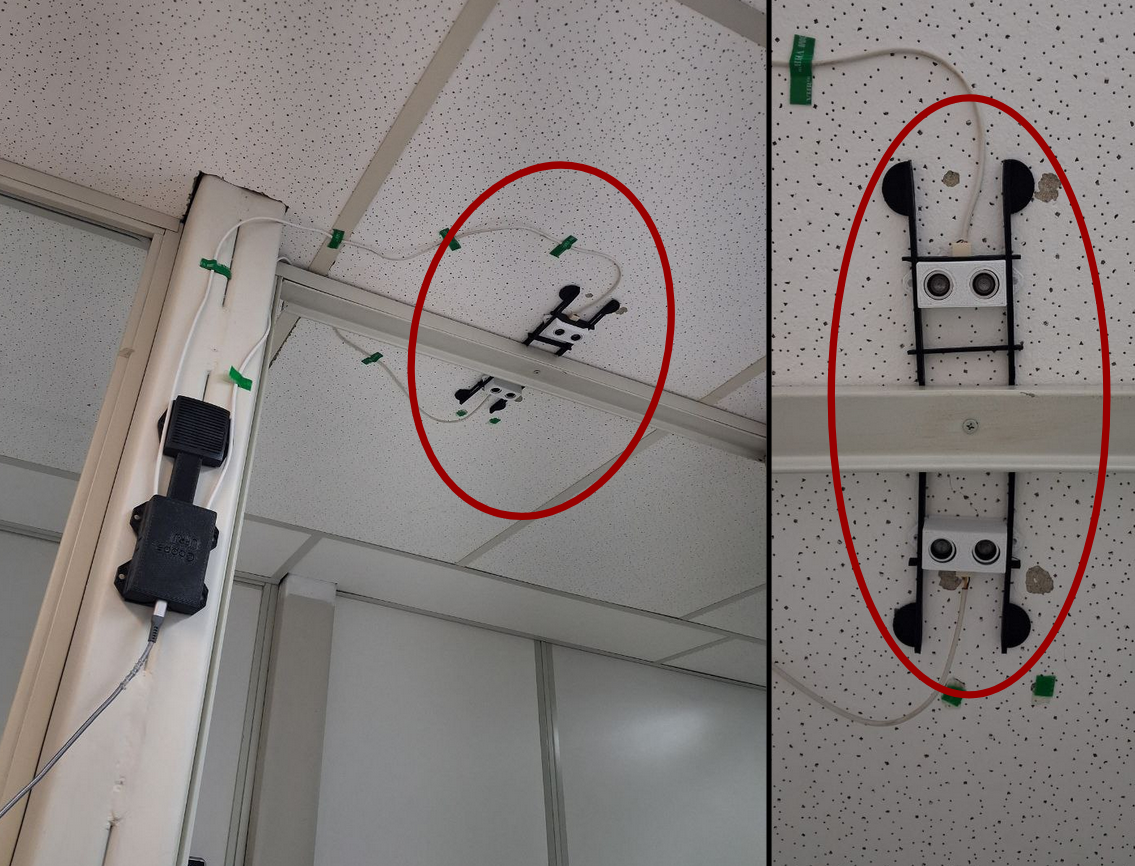
\includegraphics[scale=0.3]{images/count_people_module.png}
    \caption{Módulo de Sensoriamento para Contagem de Pessoas}
    \label{fig:count_people_module}
\end{figure}

O primeiro algoritmo proposto, para monitorar a quantidade de indivíduos em uma instalação baseia-se principalmente na disposição dos sensores ultrassônicos, que pode ser observada na Figura \ref{fig:count_people_module}, e no caráter periódico da coleta de dados pelo dispositivo IoT. Por este motivo, para cada evento de entrada ou saída, a sequência de dados coletados possui padrões bem definidos de ativação dos sensores. No caso de uma entrada, o sensor externo será ativado antes do sensor interno, bem como será o primeiro a ser desativado, para eventos de saída, o contrário acontece. Deste modo, o rastreamento de eventos de interesse, torna-se uma tarefa de identificação de padrões de ativação dos sensores.

Para lidar com este objetivo, o algoritmo construído consiste primeiramente na binarização dos dados coletados através de um limite preestabelecido, para que os estados dos sensores (ativado ou desativado) sejam diferenciados, assim como apresentado no Algoritmo \ref{alg:people_counting}. Após a binarização, o algoritmo compara o estado atual(tupla constituída pelo valor binarizado de cada sensor) com o estado anterior, para identificar e armazenar toda mudança de estado. Este novo estado, é armazenado em uma janela deslizante de tamanho fixo e a última tupla armazenada é descartada. Por fim, para cada novo estado, o algoritmo realiza a comparação entre a janela deslizante e os padrões de entrada e saída, buscando caracterizar e contabilizar eventos de interesse. Todos este fluxo pode ser visualizado através do Algoritmo \ref{alg:people_counting}.


% ------------------------------------------------------------
% No corpo do documento:


\begin{algorithm}[H]
\caption{Lógica Inicial Para Contagem de Pessoas}
\label{alg:people_counting}
\begin{algorithmic}[1]

\Function{COMPARAR\_VETORES}{$A,\;B$}
  \State \Comment{$A$ e $B$ são vetores}
  \If{$|A| \ne |B|$}  \Comment{Compara se os vetores possuem o mesmo tamanho}
    \State \Return \textbf{false}
  \EndIf

	\For{$i \gets 1$ \textbf{to} $|A|$} \Comment{Compara o valor de cada item dos vetores}
    \If{$A[i] \ne B[i]$}
      \State \Return \textbf{false}
    \EndIf
  \EndFor

	\State \Return \textbf{true} \Comment{Verdadeiro caso os vetores sejam iguais}
\EndFunction

\vspace{0.8em}

\Function{CALCULAR\_NUMERO\_DE\_PESSOAS}{$M$}
  \State $PADRAO\_DE\_ENTRADA$ \gets $[(0,0),(0,1),(1,1),(1,0),(0,0)]$
  \State $PADRAO\_DE\_SAIDA$ \gets $[(0,0),(1,0),(1,1),(0,1),(0,0)]$
  \State \Comment{$M$ é o vetor de medidas brutas}
	\State $estado\_do\_sensor \gets (s_{interno},s_{externo})$ \Comment{Vetor que armazena o estado atual binarizado}
  \State $entrada \gets 0$
  \State $saida \gets 0$
  \State $TOLERANCIA \gets 60$ \Comment{Limite para a binarização}
  \State $W \gets [(0,0),(0,0),(0,0),(0,0),(0,0)]$ \Comment{Vetor para o espaço de estados}

  \For{\textbf{each} $m \in M$}
    \State \Comment{--- Etapa de binarização das medidas brutas---}
    \If{$m.distancia\_sensor\_interno < TOLERANCIA$}
      \State $s_{interno} \gets 1$
    \Else
      \State $s_{interno} \gets 0$
    \EndIf

    \If{$m.distancia\_sensor\_externo < TOLERANCIA$}
      \State$s_{externo} \gets 1$
    \Else
      \State $s_{externo} \gets 0$
    \EndIf

    \State \Comment{--- Etapa de construção do padrão de bits capturado ---}
    \If{\textbf{not} \Call{COMPARAR\_VETORES}{$estado\_do\_sensor,\;W[5]$}}
      \State \Call{SHIFT\_LEFT}{$W$} \Comment{Descarta estado antigo}
      \State $W[5] \gets estado\_do\_sensor$ \Comment{Armazena o novo estado na última posição}

      \State \Comment{--- Etapa de identificação do evento de interesse ---}
      \If{\Call{COMPARAR\_VETORES}{$W,\;PADRAO\_DE\_ENTRADA$}}
        \State $entrada \gets entrada + 1$
      \ElsIf{\Call{COMPARAR\_VETORES}{$W,\;PADRAO\_DE\_SAIDA$}}
        \State $saida \gets saida + 1$
      \EndIf
	\State \Comment{Padrões inválidos não geram contagem}
    \EndIf
  \EndFor

  \State \Return $(entrada, saida)$
\EndFunction

\end{algorithmic}
\end{algorithm}

A lógica existente no Algoritmo \ref{alg:people_counting} faz uso da discretização dos dados e análise de mudança de estados dos sensores, para realizar tarefa de contagem de indivíduos por meio da coleta de medidas com sensores ultrassônicos, essas são ideias centrais para este tipo de atividade. No entanto, a abordagem descrita apresentou problemas durante testes práticos de funcionalidade, tendo como principal fator de seu mal funcionamento, a inexistência de uma etapa de pré-tratamento das medidas coletadas. 

Sendo assim, qualquer ruído de leitura pode induzir o sistema a gerar um estado incorreto, invisibilizando eventos de interesse e resultando em um monitoramento impreciso acerca da contagem de indivíduos em uma instalação. Ademais, o sistema de software IoT SAFE/UFRJ, tem como uma de suas principais características, a utilização de sensores de baixo custo, para construção dos dispositivos encarregados de realizar a coleta de dados \cite{SAFE-IOT}, esta categoria de sensor tende a ser mais imprecisa e ruidosa \cite{Komorowski2016}, por este motivo o sistema deve ser resiliente a este tipo de problema.

Antes de tratar ruídos e valores discrepantes (\textit{outliers}), é necessário compreender o verdadeiro gerador deste tipo de informação. Isto se faz necessário, pois este tipo de dado pode fornecer informações úteis para a etapa de modelagem do problema, bem como a exclusão de informações importantes de forma errônea pode comprometer todo o conjunto de dados inserindo viés ou simplesmente desperdiçando informações importantes \cite{Komorowski2016}. Logo, a segunda etapa do processo de evolução do módulo de contagem de pessoas, consiste na coleta e análise exploratória dos dados, para que se possa compreender e reconhecer os padrões naturais presentes na informação coletada \cite{Komorowski2016}.



%% Fim da seção do módulo existente e limitações

%%Inicio da seção de análise exploratória
\subsection{Análise Exploratória dos Dados}
\label{subsec:exploratory_data_analysis}

A visualização gráfica é um método para análise de dados, que permite apresentar características como dispersão e padrões de comportamento, apenas através de dados coletados \cite{wohlin2012experimentation}. A etapa de coleta, consistiu na elaboração de um roteiro que cobrisse todos os possíveis eventos de entrada e saída de um indivíduo em uma instalação, para isso foi elaborado a Tabela \ref{tab:events_description}, que apresenta a numeração de cada evento e sua descrição. Este processo fez-se necessário, pois foi observado maior variação dos dados em eventos que envolviam a interação do indivíduo com a porta da instalação, uma vez que os sensores também captam o movimento da porta.

\renewcommand{\arraystretch}{1.3}
\begin{table}[H]
	\centering
	\caption{Roteiro de Eventos para Etapa de Coleta de Dados}
	\label{tab:events_description}
	\begin{tabular}{|c|c|l|}
		\hline
		\multicolumn{1}{|l|}{\textbf{Evento}} & \multicolumn{1}{l|}{\textbf{Estado Inicial da Porta}} & \multicolumn{1}{c|}{\textbf{Descrição}}                    \\ \hline
		1                                     & Fechada                                               & Abrir a porta, realizar a entrada e fechar a porta.        \\
		2                                     & Fechada                                               & Abrir a porta, realizar a saída e fechar a porta.          \\
		3                                     & Fechada                                               & Abrir a porta, realizar a entrada e manter a porta aberta. \\
		4                                     & Fechada                                               & Abrir a porta, realizar a saída e manter a porta aberta.   \\
		5                                     & Aberta                                                & Realizar a entrada e manter a porta aberta.                \\
		6                                     & Aberta                                                & Realizar a saída e manter a porta aberta.                  \\
		7                                     & Aberta                                                & Realizar a entrada e fechar a porta.                       \\
		8                                     & Aberta                                                & Realizar a saída e fechar a porta.                         \\ \hline
	\end{tabular}
\end{table}

O roteiro de coleta de dados foi executado com seis indivíduos diferentes para que se pudesse observar variações e dispersões em função dos indivíduos e da forma de entrada ou saída de cada um. Para facilitar estas observações, cada evento realizado possui uma gravação de vídeo correspondente, que atua como registro auxiliar durante a etapa de análise dos dados. Desta forma, todo o processo torna-se mais auditável, tendo em vista que o evento armazenado pode ser revisto, ajudando na melhor compreensão de ruídos e \textit{outliers}. A Figura \ref{fig:data_collect} apresenta um conjunto de imagens acerca dos registros de vídeo.

\begin{figure}[ht]
    \center
    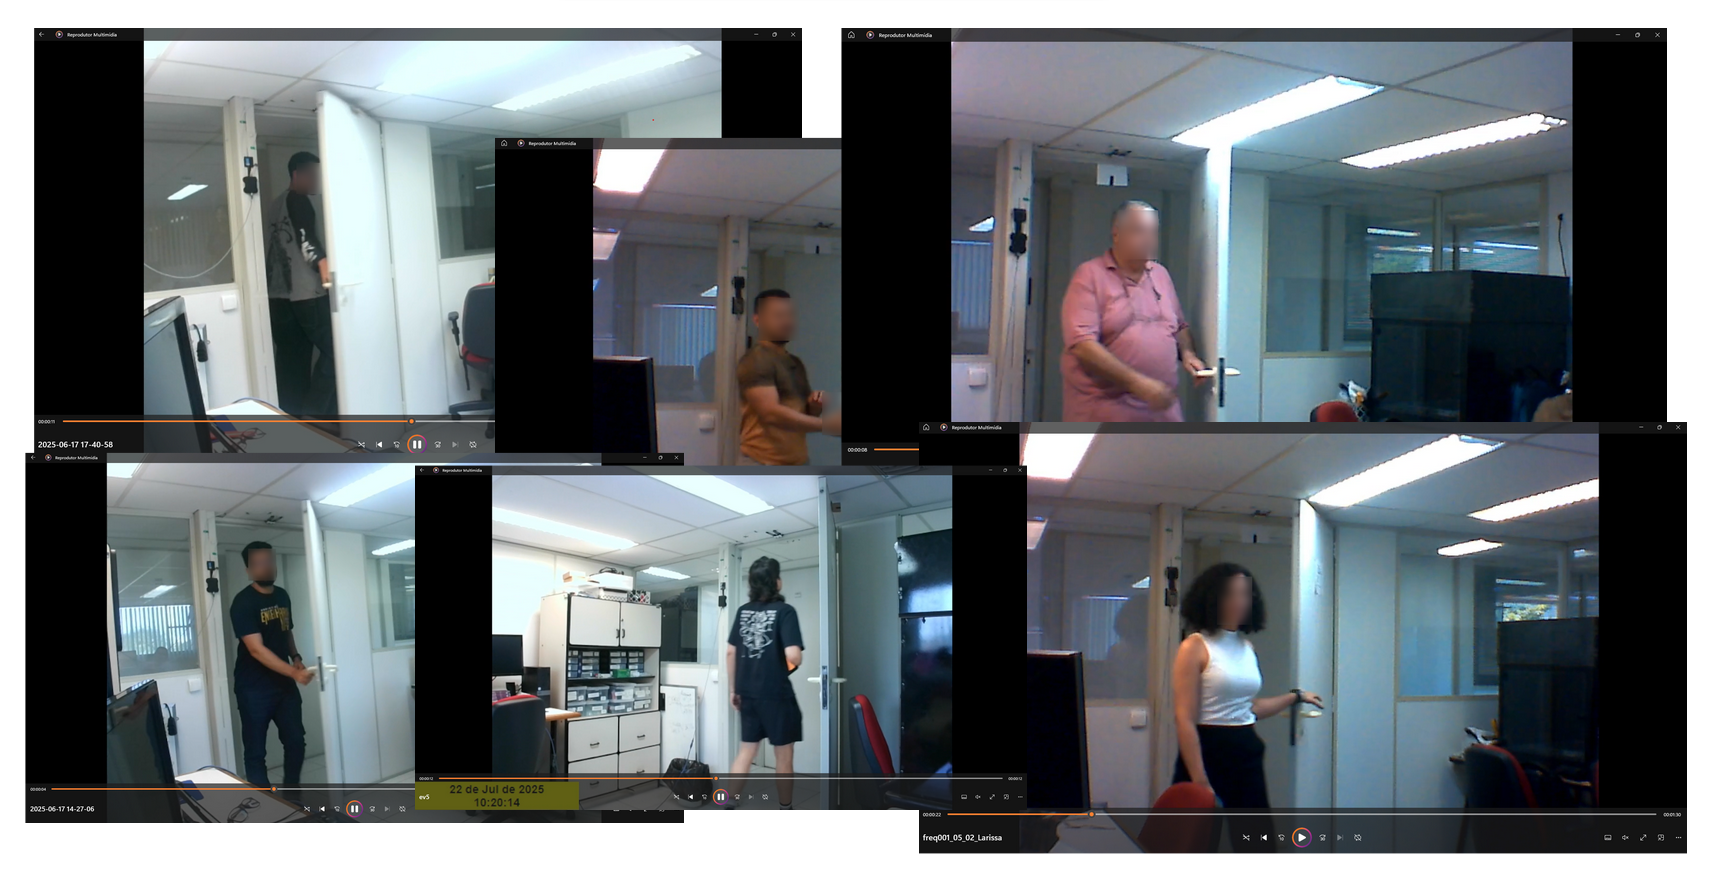
\includegraphics[scale=0.25]{images/data_collect.png}
    \caption{Registros de vídeo realizados durante a coleta de dados}
    \label{fig:data_collect}
\end{figure}

Para a etapa de construção das visualizações gráficas, empregou-se predominantemente a técnica de gráficos bidimensionais de pontos e linhas, conforme ilustrado na Figura \ref{fig:data_visualization}. Essas visualizações representam graficamente os valores de um vetor no eixo y em função de intervalos regulares no eixo x \cite{Komorowski2016}. No contexto da Figura \ref{fig:data_visualization}, o eixo y apresenta os valores de distância medidos pelos sensores ultrassônicos, enquanto o eixo x corresponde ao instante temporal de cada coleta. Além disso, essa abordagem foi adotada pois, em conjunto com os registros de vídeo, permite auditar individualmente cada amostra coletada (representada por um ponto no gráfico), possibilitando a identificação visual de inconsistências, anomalias e medições claramente incompatíveis com o cenário físico observado.


\begin{figure}[H]
    \center
	\fbox{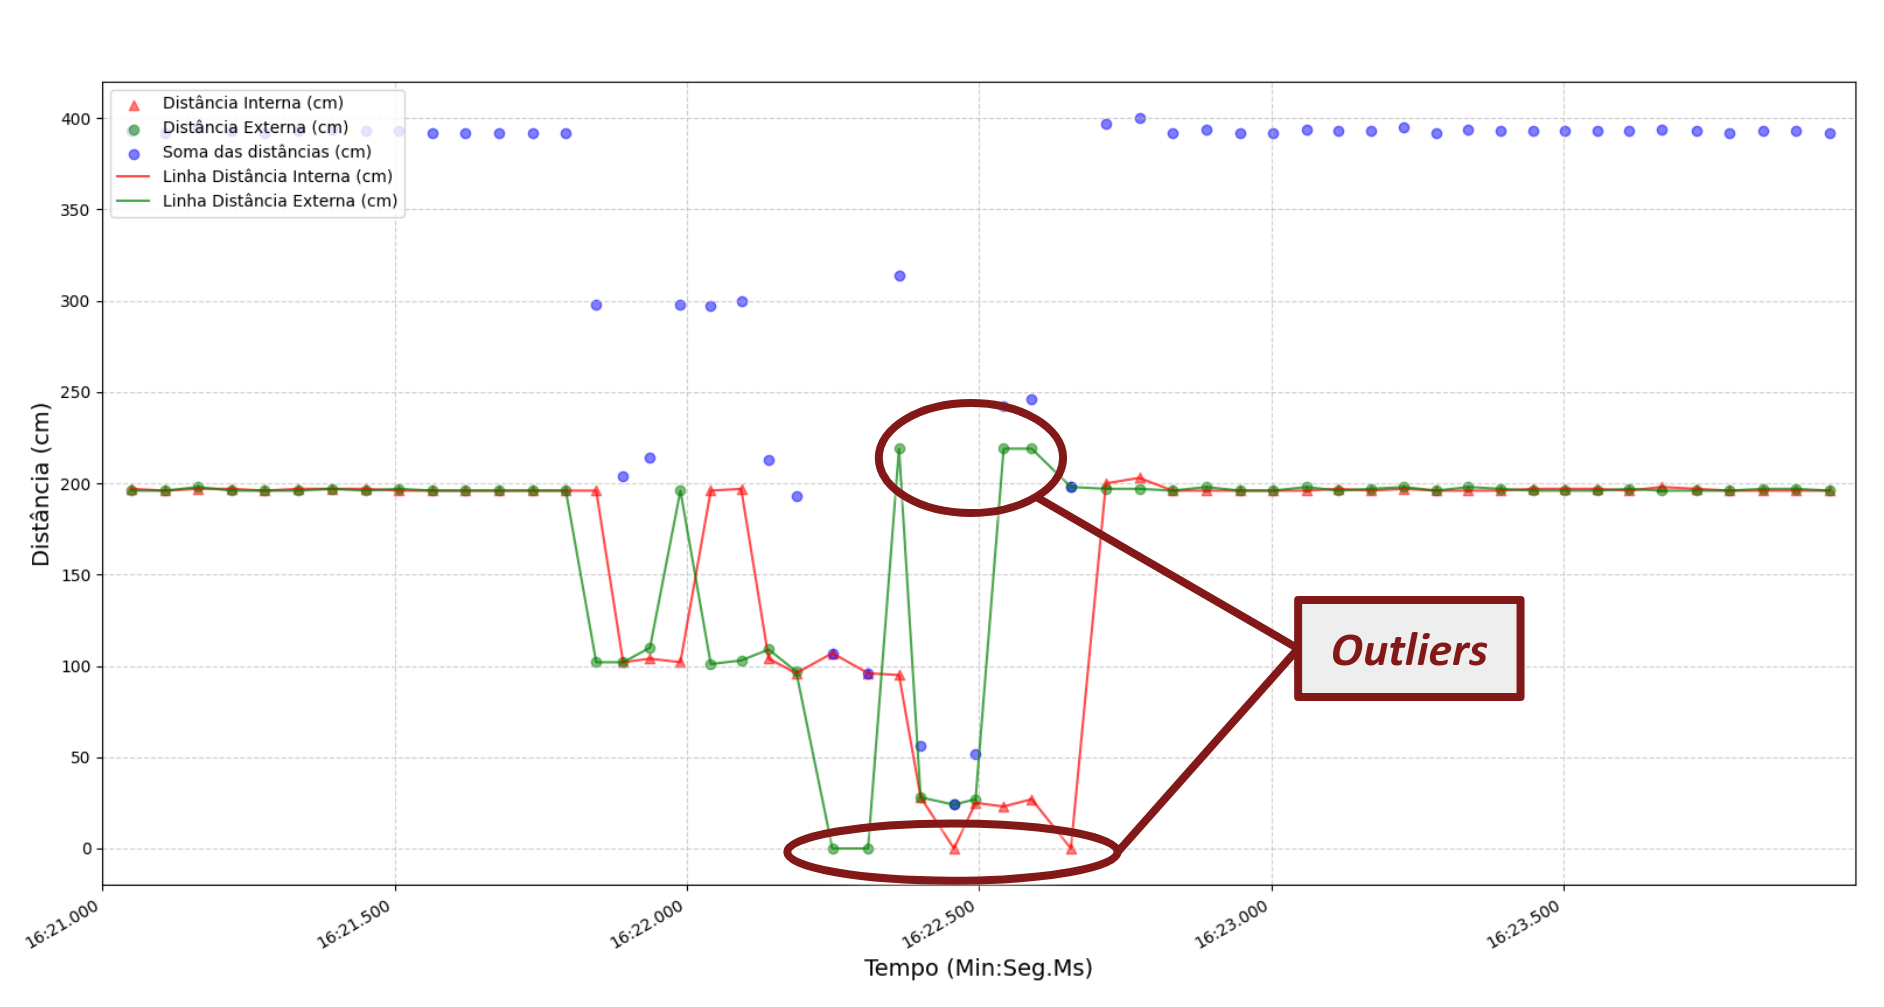
\includegraphics[scale=0.22]{images/datapoints_visualization.png}}
	\caption{Visualização gráfica de um evento de entrada}
	\label{fig:data_visualization}
\end{figure}

A etapa de análise visual dos gráficos apresentou dois padrões de \textit{outliers}, valores superiores a distância total entre os sensores ultrassônicos e o piso, isto é, registros que deveriam ser impossíveis de serem coletados e também valores nulos. O primeiro padrão pode ser justificado devido a interferência entre os dois sensores. Já a ocorrência de valores nulos acontece quando o sensor não consegue captar a onda enviada, isto pode acontecer quando um objeto ou indivíduo impede a propagação da onda, e também caso a onda não seja captada pelo receptor, ocorrência mais comum em objetos com faces irregulares, pois a onda pode ser refletida em direções que não são paralelas ao seu vetor deslocamento inicial, dificultando sua recepção pelo sensor que apenas consegue captar informações em uma região cônica de aproximadamente 45 graus \cite{hcsr04}. 

Além disso, compreende-se que um dos motivos de mal funcionamento do Algoritmo \ref{alg:people_counting} corresponde a ausência de abordagens para lidar com comportamentos irregulares advindos da natureza do sensor utilizado e da estratégia de coleta. A propagação da onda por trajetórias indesejadas é um problema de difícil resolução, tendo em vista que o indivíduo encontra-se em movimento e pode ser interceptado por diversos ângulos. No entanto, existem vários ajustes que podem ser realizados para melhorar a qualidade do evento capturado e consequentemente aprimorar a caracterização pelo sistema. Sendo assim, foram realizados testes para identificar customizações de caráter lógico e físico, que refinassem a coleta de informações, culminando na obtenção de padrões mais constantes e livres de irregularidades. 

\begin{figure}[H]
	\centering

	% --- Primeira linha ---
	\begin{subfigure}[b]{0.48\textwidth}
		\centering
		\fbox{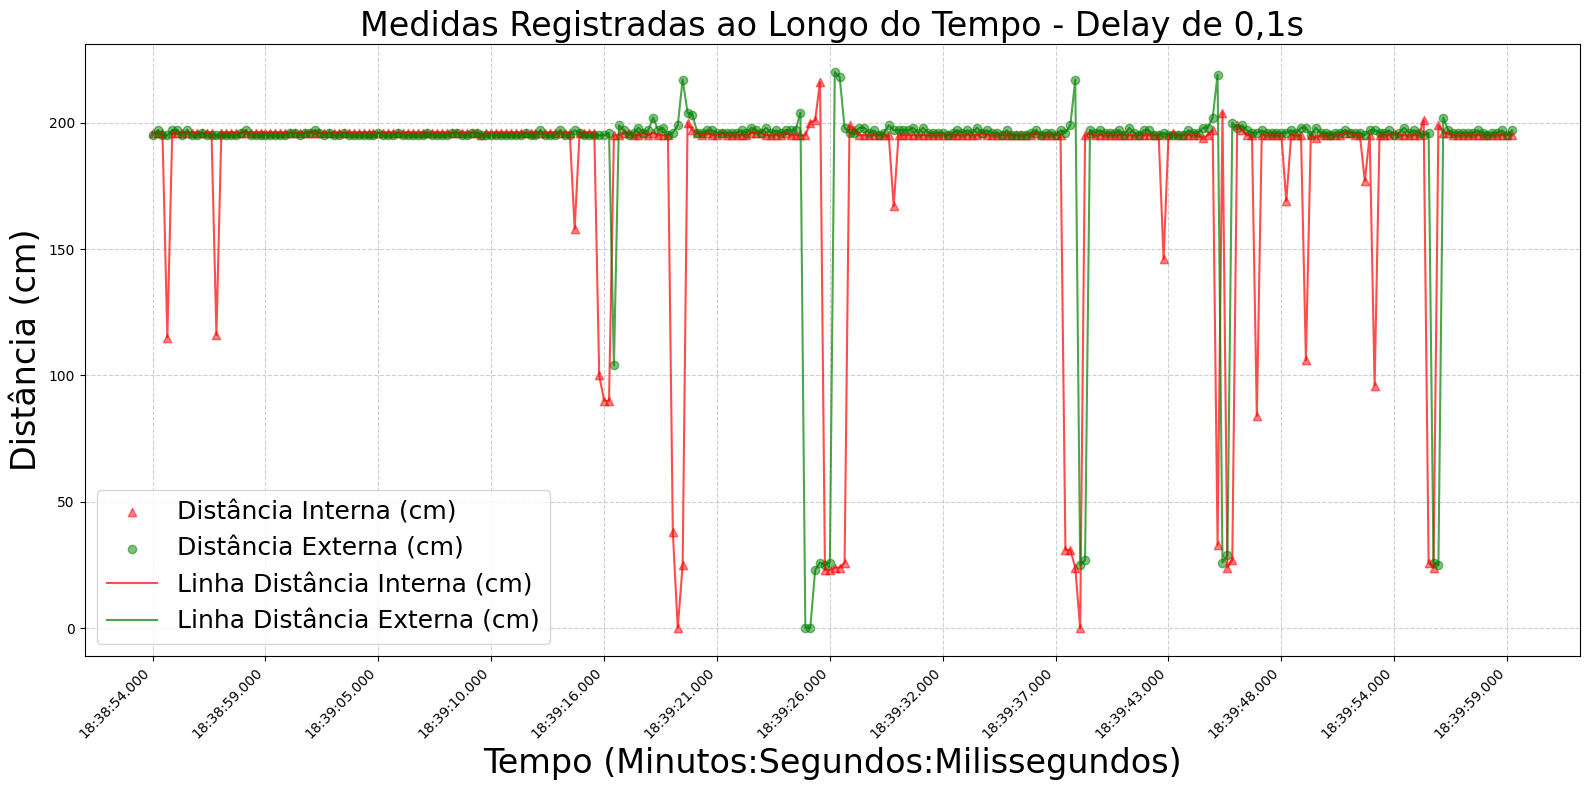
\includegraphics[width=\textwidth]{images/noise_freq_01.png}}
		\caption{Intervalo de 0,1 segundos}
		\label{fig:noise_analysis_01}
	\end{subfigure}
	\hfill
	\begin{subfigure}[b]{0.48\textwidth}
		\centering
		\fbox{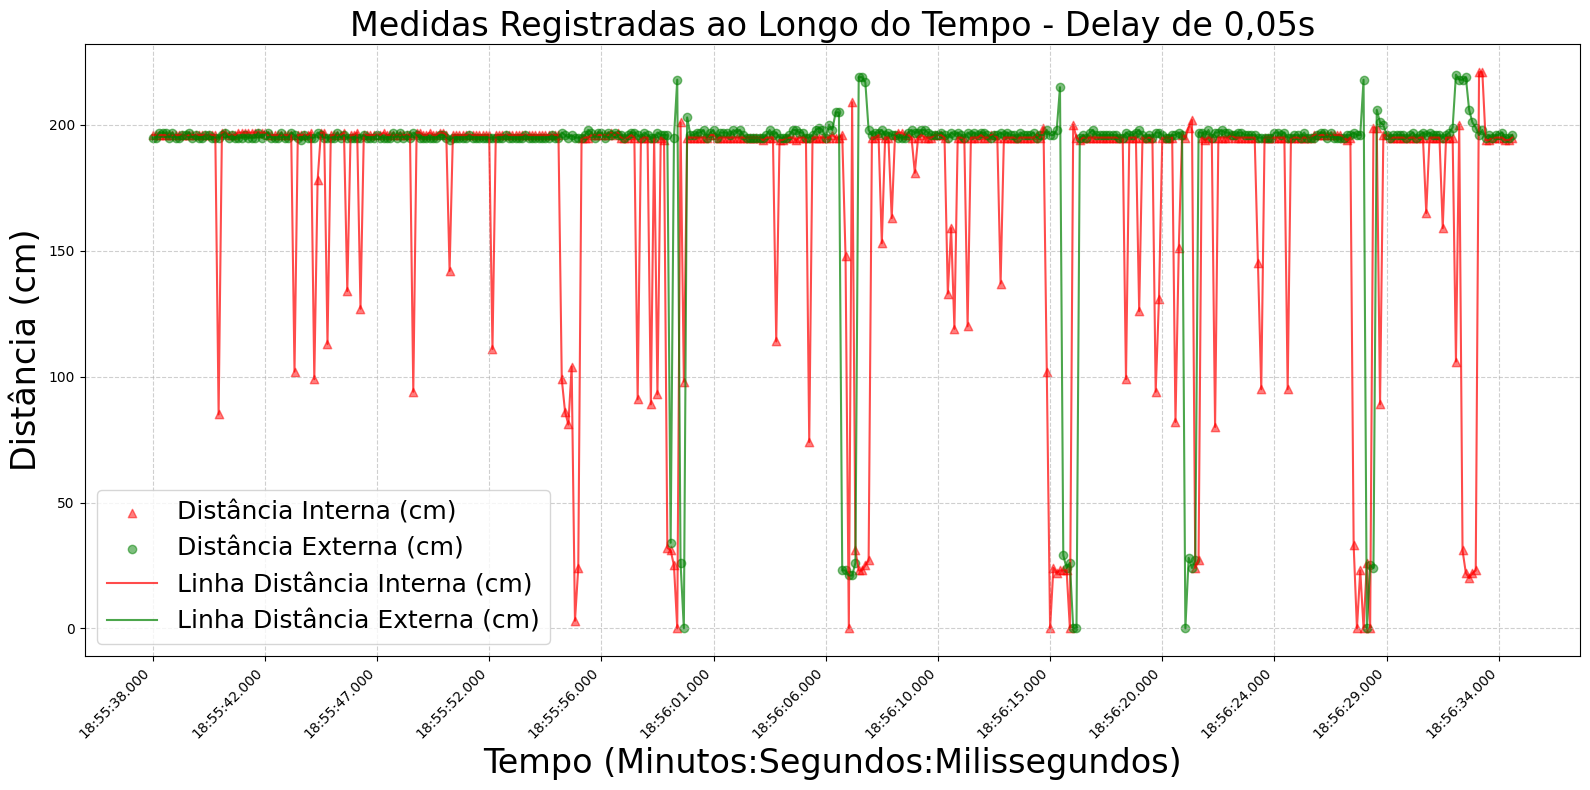
\includegraphics[width=\textwidth]{images/noise_freq_005.png}}
		\caption{Intervalo de 0,05 segundos}
		\label{fig:noise_analysis_005}
	\end{subfigure}

	\vspace{0.4cm}

	% --- Segunda linha ---
	\begin{subfigure}[b]{0.48\textwidth}
		\centering
		\fbox{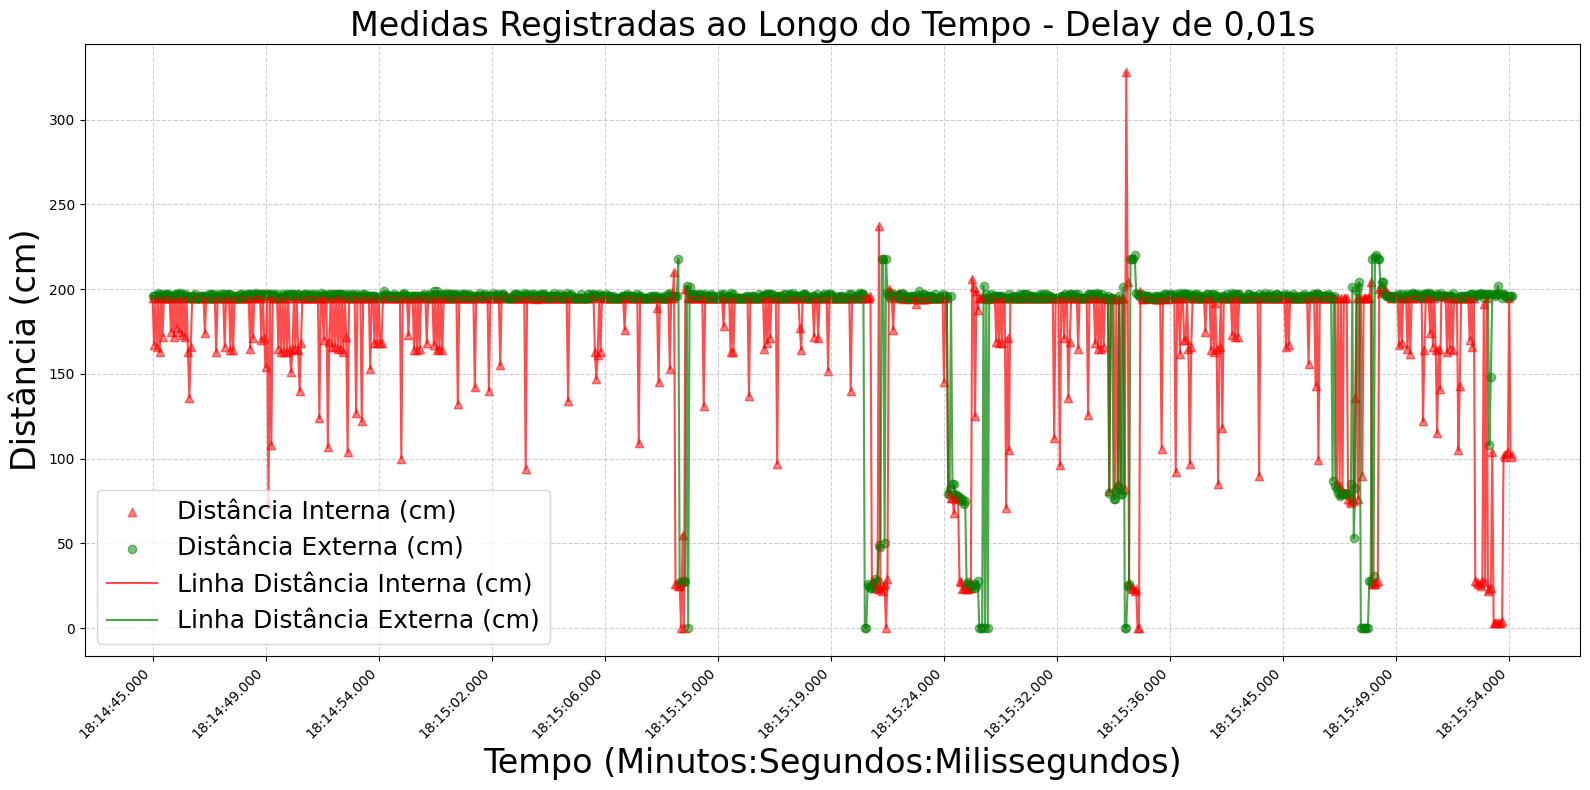
\includegraphics[width=\textwidth]{images/noise_freq_001.png}}
		\caption{Intervalo de 0,01 segundos}
		\label{fig:noise_analysis_001}
	\end{subfigure}

	\caption{Coleta de dados realizadas com intervalos de medição diferentes}
	\label{fig:noise_analysis}
\end{figure}


A fim de determinar o intervalo de coleta que minimiza a interferência entre os sensores, foi realizado uma série de testes com o mesmo dispositivo e nas mesmas condições físicas. Para cada ensaio, variou-se o tempo de espera de cada sensor antes de realizar a sequência de medições. A Figura \ref{fig:noise_analysis} apresenta três gráficos, um para cada intervalo testado, pode-se observar, que ao diminuir o tempo de espera para coleta entre cada sensor, o ruído aumenta de forma quase proporcional. Esse aumento ocorre, pois com um intervalo mais curto a onda emitida por um dos sensores não possui tempo suficiente para se dissipar antes que o outro sensor inicie sua coleta, como as ondas possuem mesma frequência, os sensores não conseguem realizar uma distinção entre elas. Logo, como a distância coletada é calculada através do tempo de deslocamento, caso o sensor receba uma onda que não foi emitida por ele, o valor interpretado será incorreto, pois o \textit{hardware} não sabe lidar com este tipo de situação. 

No entanto, intervalos muito grandes também são um problema, porque a quantidade de dados coletados pode ser insuficiente para categorizar os eventos de interesse. Por fim, o valor adotado foi o de 0,05 segundos, uma vez que apresentou grande diminuição no ruído se comparado ao gráfico de intervalos de 0,01 segundos, bem como obteve caracterização satisfatória de eventos de interesse, diferentemente do gráfico com intervalos de 0,1 segundos.

Outro problema a ser analisado, consiste na dificuldade em identificar eventos de interesse e definir o início e fim destas ocorrências, para posterior análise. Como apresentado nas Figuras \ref{fig:data_visualization} e \ref{fig:noise_analysis} as medidas coletadas não estão livres de interferência entre os sensores, logo a caracterização de eventos de interesse pode ser comprometida. Para lidar com esta problemática, foi acrescentado a parte física do sistema, uma divisória que é anexada a porta da instalação. Sendo assim, sempre que a porta se encontra fechada, a divisória reduz o alcance das ondas propagadas por um dos sensores, retornando sempre uma distância fixa, algo que facilita a busca por padrões de inatividade do sistema. Portanto, ao buscar eventos interesse, basta analisar conjuntos de dados que não correspondem a períodos de inatividade, esta solução facilita a caracterização e poupa processamento, tendo em vista que o sistema não precisa realizar uma análise contínua das medidas coletadas.

Por fim, conclui-se através da análise exploratória dos dados, que o mal funcionamento do módulo de contagem de pessoas corresponde a dois principais fatores: (i) dificuldade em identificar e delimitar conjuntos de dados que compreendam eventos de interesse; (ii) a interferência entre os sensores devido a características inerentes à seu funcionamento. Logo, para que o módulo seja evoluído e seu desempenho aprimorado, deve-se adotar métodos para lidar com estes fatores. 


%%Fim da seção de análise exploratória

%%Início da seção de abordagem proposta
\subsection{Evolução do Módulo e Estratégia de Contagem}
\label{subsec:module_evolution}

As etapas descritas anteriormente foram imprescindíveis, para delinear pontos fracos acerca do módulo de contagem de pessoas existente e através da visualização e análise dos dados, compreender como este componente do sistema pode ser evoluído. Sendo assim, a presente subseção pretende apresentar uma sequência de etapas que compõe a nova estratégia utilizada para contagem de indivíduos pelo sistema, que tem como principal objetivo suprir as necessidades destacadas anteriormente, como lidar de melhor forma com a interferência entre os sensores e identificar possíveis eventos de interesse com mais assertividade.

\begin{figure}[H]
    \center
    \fbox{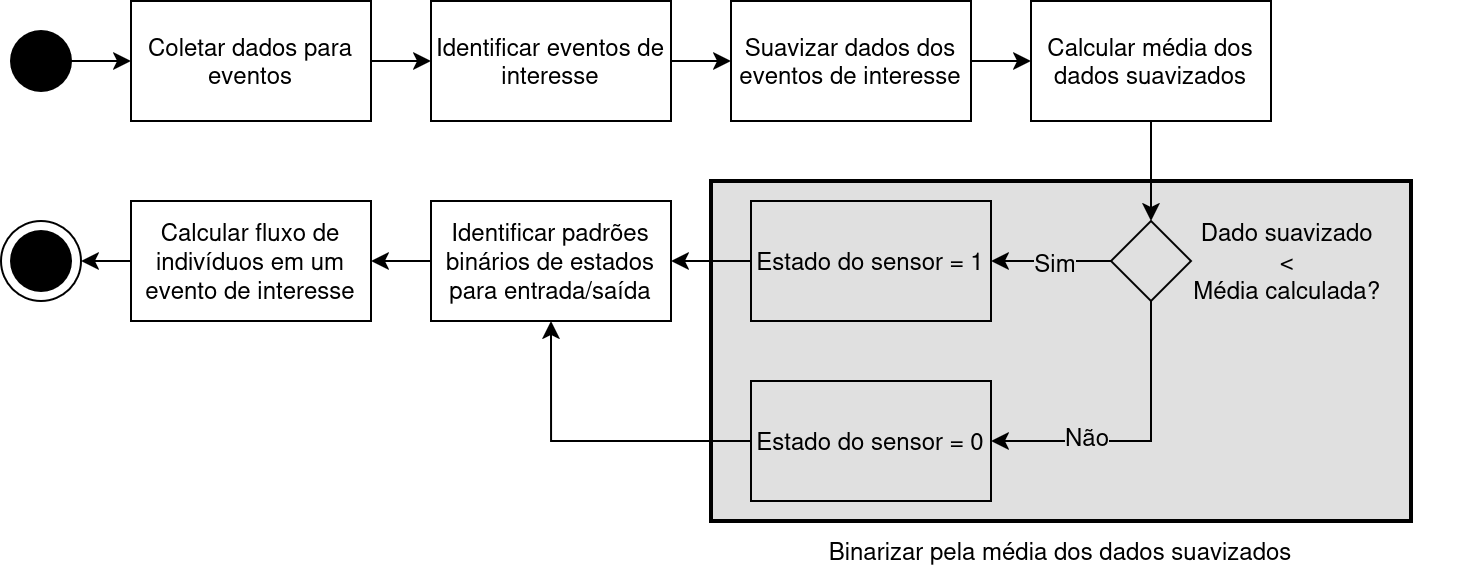
\includegraphics[width=\linewidth]{images/fluxo_new_approach.png}}
    \caption{Fluxo de procedimentos para o cálculo de fluxo de pessoas em um evento}
    \label{fig:strategy_workflow}
\end{figure}

A Figura \ref{fig:strategy_workflow} apresenta de forma sucinta, o fluxo de etapas que compõem o processo de contagem de indivíduos pelo sistema. Em contraste ao Algoritmo \ref{alg:people_counting} pode-se observar a adoção de duas novas etapas de pré-processamento, agregar medidas e suavizar dados coletados. Além disso, a discretização por meio da criação de estados de ativação(ativo ou inativo) foi mantida, no entanto a estratégia para obtenção do limite de binarização foi evoluída, para que esse valor seja obtido de forma dinâmica para cada evento detectado pelo sistema, ou seja, para cada conjunto de dados coletados.

O processo de identificar uma sequência de dados que podem conter um evento de interesse, consiste em uma tarefa difícil como destacado em parágrafos anteriores, mais especificamente delimitar seu início e fim, tendo em vista que a interferência causada entre os sensores gera variações abruptas nos dados coletados, assim como apresentado na Figura \ref{fig:noise_analysis}. Para lidar com este tipo de comportamento, foi adicionado a etapa de agregação de medidas, que consiste apenas na soma das leituras realizadas pelo sensor externo e interno, gerando um novo tipo de informação, que é utilizado para identificar medidas que correspondem há um evento de interesse. A lógica para seu uso é muito simples, durante períodos de inatividade, isto é, que não há nenhum indivíduo entrando ou saindo da instalação, a soma das leituras deve estar compreendida em um intervalo fixo e não deve variar muito. O motivo para este comportamento consiste no fato de que, períodos de inatividade correspondem a observação de eventos estáticos, que por sua natureza  apresentam dados mais regulares, esta característica pode ser observada através dos pontos azuis presentes na Figura \ref{fig:data_collect}. Deste modo, por exclusão, pode-se concluir que apenas medidas que não se encaixam nestes parâmetros podem representar eventos de interesse. Esta abordagem é utilizada para separar e armazenar conjuntos de dados que não necessariamente retratam este tipo de evento, mas que são grandes candidatos para tal.

Mesmo após a identificação de conjuntos de dados que possam conter eventos de interesse, ainda é necessário lidar com problemas causados pela interferência entre os sensores, tendo em vista que, a existência de medidas incorretas pode impedir que o sistema identifique e contabilize uma entrada ou saída. Por este motivo, a próxima etapa após a construção destes conjuntos consiste na suavização dos dados coletados, é possível utilizar esta abordagem, pois o sistema coleta medidas com uma frequência alta, logo por mais que existam dados incorretos, outros pontos em sua vizinhança tem influência acerca do valor daquela medida, impedindo que ela corresponda a valores com grande variação. 

\begin{figure}[H]
    \centering

    % --- Primeira linha ---
    \begin{subfigure}[b]{0.48\textwidth}
        \centering
	    \fbox{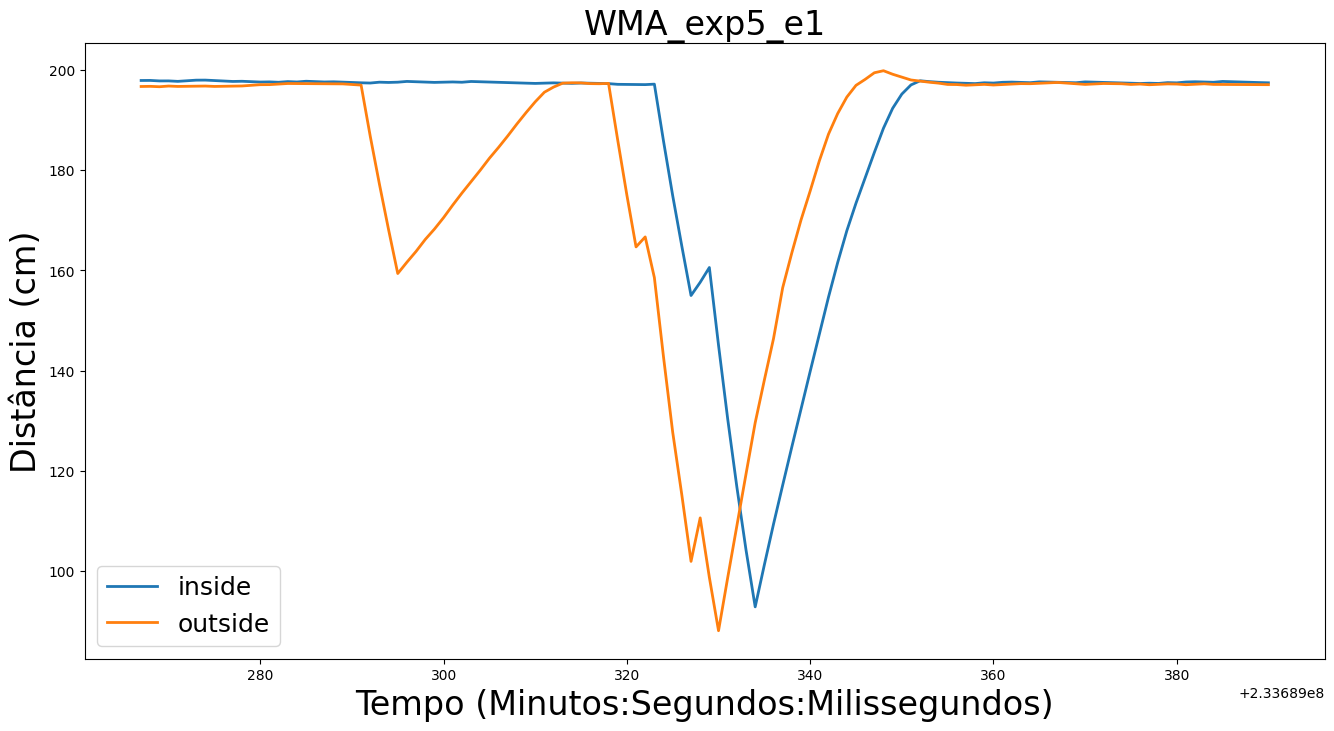
\includegraphics[width=\textwidth]{images/wma_plot.png}}
        \caption{Suavização utilizando Médias Móveis com Peso}
        \label{fig:wma_smooth}
    \end{subfigure}
    \hfill
    \begin{subfigure}[b]{0.48\textwidth}
        \centering
	    \fbox{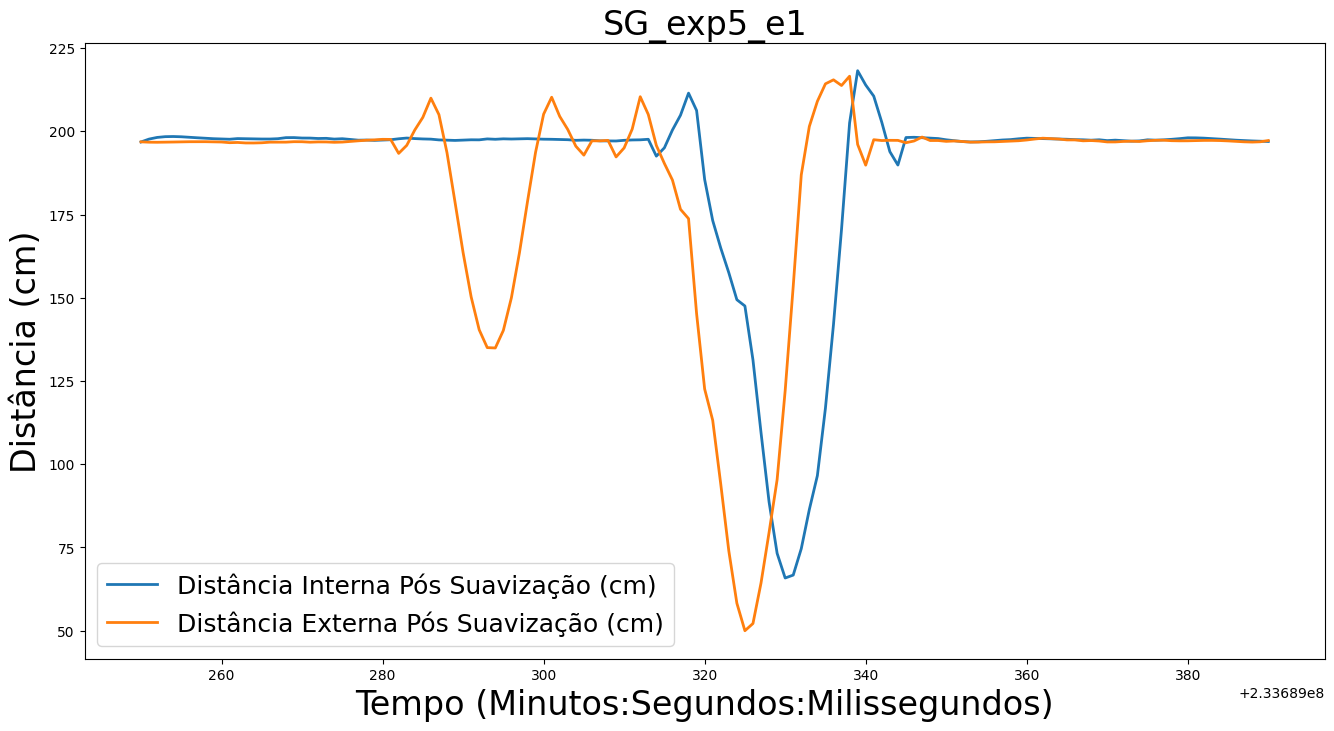
\includegraphics[width=\textwidth]{images/savgol_plot.png}}
        \caption{Suavização utilizando Savitzky-Golay}
        \label{fig:savgol_smooth}
    \end{subfigure}

    \vspace{0.4cm}

    % --- Segunda linha ---
    \begin{subfigure}[b]{0.9\textwidth}
        \centering
	    \fbox{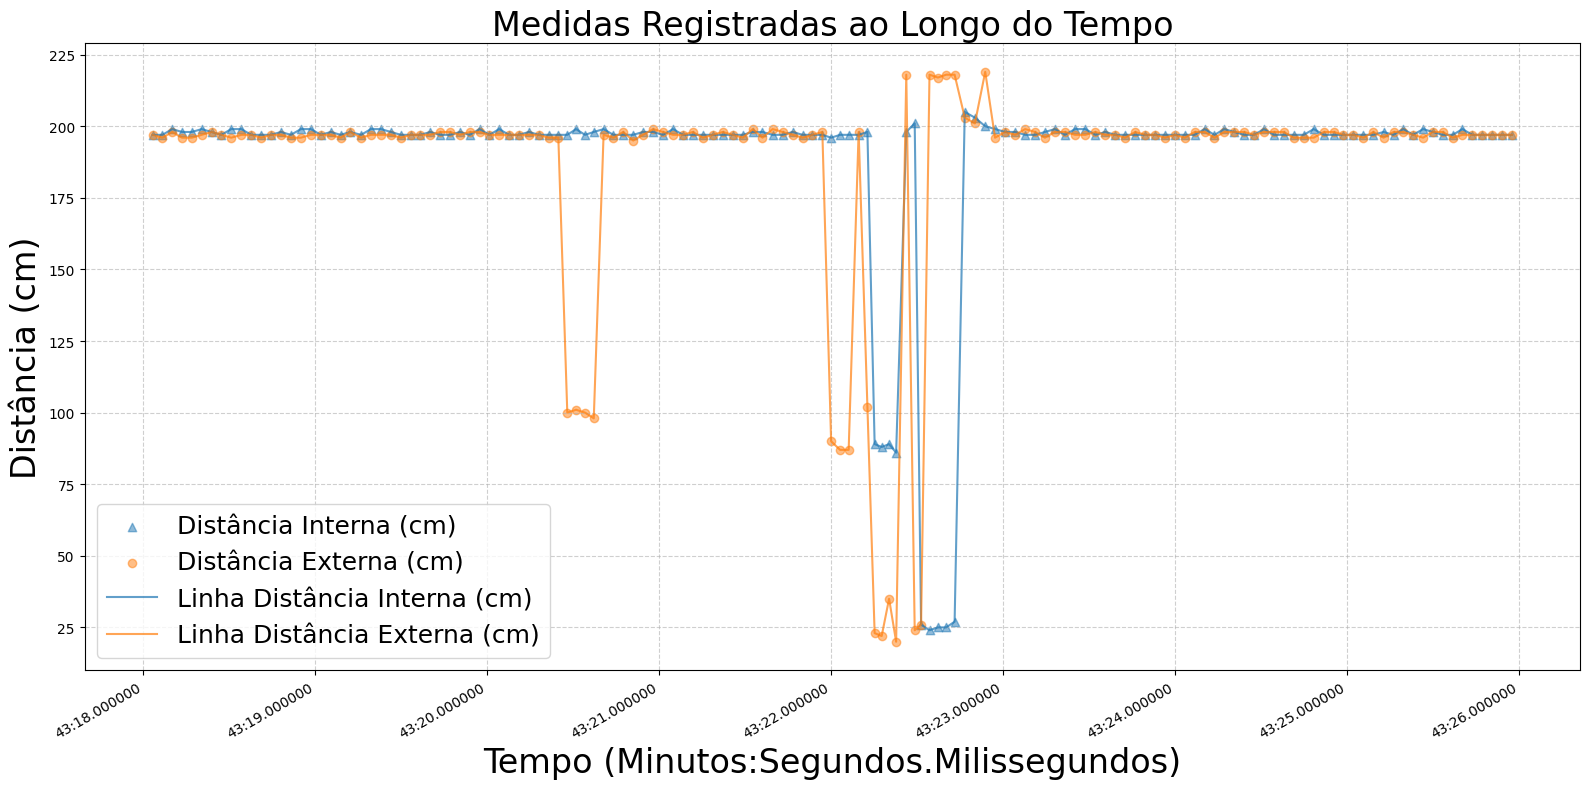
\includegraphics[width=\textwidth]{images/plot_pre_smooth.png}}
        \caption{Apresentação dos dados sem suavização das amostras}
        \label{fig:pre_smooth}
    \end{subfigure}

    \caption{Comparação entre técnicas de suavização de dados aplicadas às medições dos sensores ultrassônicos.}
    \label{fig:smoothing_analysis}
\end{figure}

A Figura \ref{fig:smoothing_analysis} apresenta duas técnicas muito comuns para suavização de dados que possuem ruído e também atenuação de sinal. Neste contexto, a Figura \ref{fig:wma_smooth} corresponde ao emprego de um algoritmo de Média Móveis com Peso (\textit{Weighted Moving Average} - WMA), uma estratégia simples que consiste na ideia de quão maior a distância entre dois pontos, menor a influência entre eles \cite{wang_time_2020}. A equação \ref{eq:wma} apresenta a definição para este tipo de abordagem, neste contexto $\omega_i$ corresponde ao peso/influência da informação presente na posição $i$ acerca do dado contido na posição $t$. Através da Figura \ref{fig:smoothing_analysis}, pode-se observar que esta abordagem gera uma série temporal livre de ruídos e fiel ao comportamento original que pode ser observado na Figura \ref{fig:pre_smooth}. No entanto por não utilizar artifícios polinomiais a representação apresenta picos e variações abruptas, este tipo de comportamento dificulta o processo de caracterização do evento de interesse entre os dados analisados, pois pode gerar falsos positivos durante a etapa de reconhecimento de padrões.

\begin{equation}
\hat{x}_t = \sum_{i=-n}^{n} \omega_i x_{i+t}
\label{eq:wma}
\end{equation}

Outro método muito comum de suavização de dados, mais especificamente no âmbito da engenharia elétrica, consiste no filtro de Savistky-Golay \cite{schafer_what_2011}, que utiliza a ideia de suavização polinomial por mínimos quadrados. Essa técnica consiste em aproximar um conjunto $2M + 1$ de amostras $x[n]$, centradas em $n=0$, por um polinômio $p(n)$ de grau $N$, cujos coeficientes são determinados de modo a minimizar a soma dos erros quadráticos entre o polinômio e as amostras, como apresentado na Equação \ref{eq:erro_sg}. O valor suavizado no ponto central é obtido avaliando o polinômio em $n = 0$, isto é, $y[0]=p[0]=a_0$.

\begin{equation}
\begin{aligned}
\mathcal{E}_N 
&= \sum_{n=-M}^{M} \left( p(n) - x[n] \right)^2 = \sum_{n=-M}^{M} \left( \sum_{k=0}^{N} a_k n^k - x[n] \right)^2
\end{aligned}
\label{eq:erro_sg}
\end{equation}


A Figura~\ref{fig:savgol_smooth} apresenta a aplicação do filtro de Savitzky-Golay ao mesmo conjunto de dados, permitindo a comparação direta com a técnica de WMA. Observa-se que o emprego de técnicas polinomiais resulta em variações mais suaves, algo vantajoso por dois motivos principais. Primeiramente, os vales passam a apresentar formas mais arredondadas e sem variações abruptas, evitando sequências do tipo vale–pico–vale, sem que seja necessário a adoção de uma grande janela de amostras, o que reduz a ocorrência de falsas mudanças no estado de ativação dos sensores e confere maior estabilidade numérica ao sistema. Além disso, nota-se a formação de regiões de decaimento após cada grande vale, o que é particularmente útil, uma vez que a definição dos estados de ativação é realizada por meio da binarização pela média dos valores coletados. Dessa forma, a existência de um tempo de decaimento contribui para uma transição mais suave e confiável entre os estados. Por este motivo, a abordagem adotada para o processo de suavização dos dados no sistema SAFE/UFRJ, foi o filtro de Savistky-Golay.

Após o processo de suavização, é realizado a binarização por limiares para que sejam determinados os estados de ativação dos sensores interno e externo para cada medida coletada. O intuito desta binarização é o mesmo presente no Algoritmo \ref{alg:people_counting}, espera-se que através de uma sequência pré-determinada de estados, seja possível identificar e contabilizar um evento de interesse. No entanto, ao aplicar o filtro de Savistky-Golay o valor numérico coletado pelos sensores é atenuado, deste modo os limites anteriores, valores constantes, não funcionam de forma tão eficaz como anteriormente. Para gerar o novo limite de binarização, é utilizado a Equação \ref{eq:media_geral_compacta}, que consiste na média aritmética entre a média das medidas externas e a média das medidas internas após a aplicação do filtro de Savistky-Golay. 

\begin{equation}
\bar{x}_{geral}
= \frac{1}{2}
\left(
	\frac{1}{N} \sum_{n=1}^{N} x_{externo}[n]
+
	\frac{1}{N} \sum_{n=1}^{N} x_{interno}[n]
\right)
\label{eq:media_geral_compacta}
\end{equation}

O valor obtido por meio da Equação~\ref{eq:media_geral_compacta} pode ser interpretado como uma estimativa do nível médio das medições realizadas pelos dois sensores e pode ser observado através da Figura \ref{fig:smoothing_ex}. Dessa forma, valores inferiores a esse limiar são associados à ativação do sensor, indicando a presença de um indivíduo ou objeto abaixo do sensor, enquanto valores superiores correspondem a inatividade. Com o objetivo de evitar ativações indevidas causadas por objetos de pequenas dimensões ou ruídos de medição, foi estabelecido um limite mínimo adicional de 50~cm, determinado de forma experimental.

\begin{figure}[H]
    \centering

    % --- Primeira linha ---
    \begin{subfigure}[b]{0.48\textwidth}
        \centering
	    \fbox{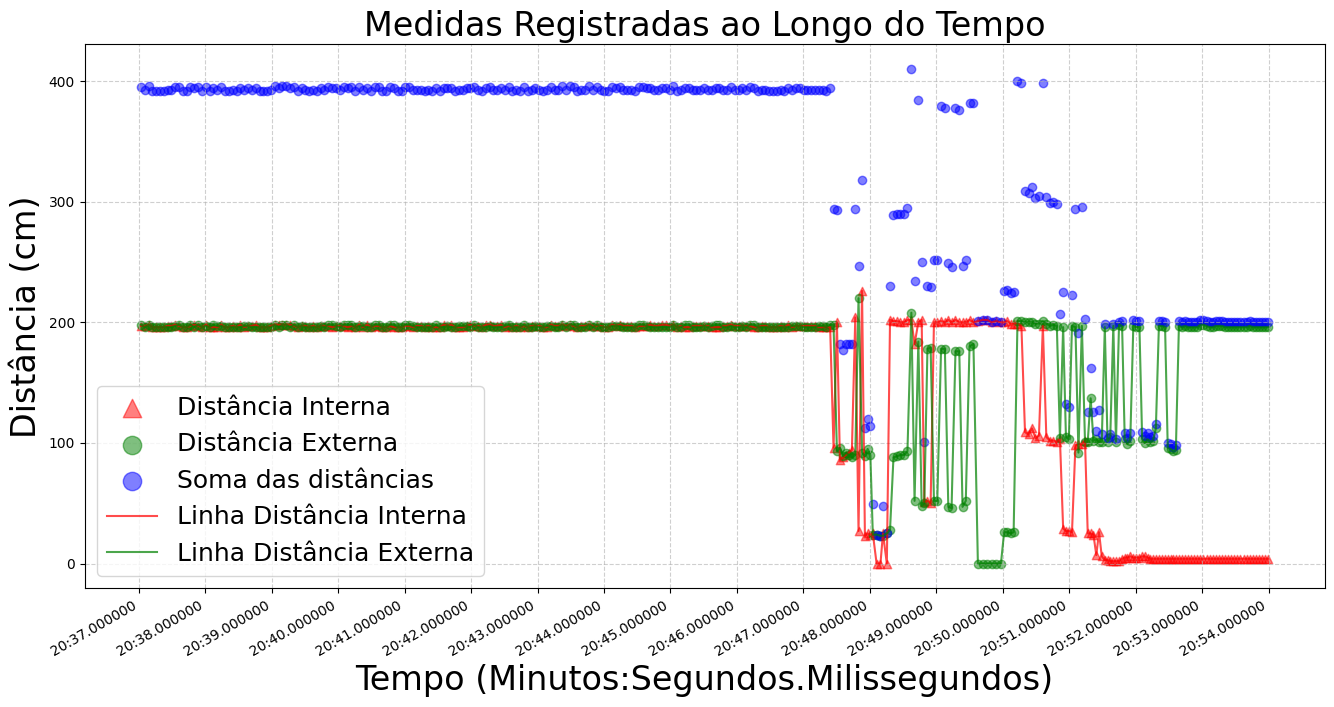
\includegraphics[width=\textwidth]{images/plot_event_ex.png}}
        \caption{Janela temporal de medidas coletadas}
        \label{fig:plot_ex}
    \end{subfigure}
    \hfill
    \begin{subfigure}[b]{0.48\textwidth}
        \centering
	    \fbox{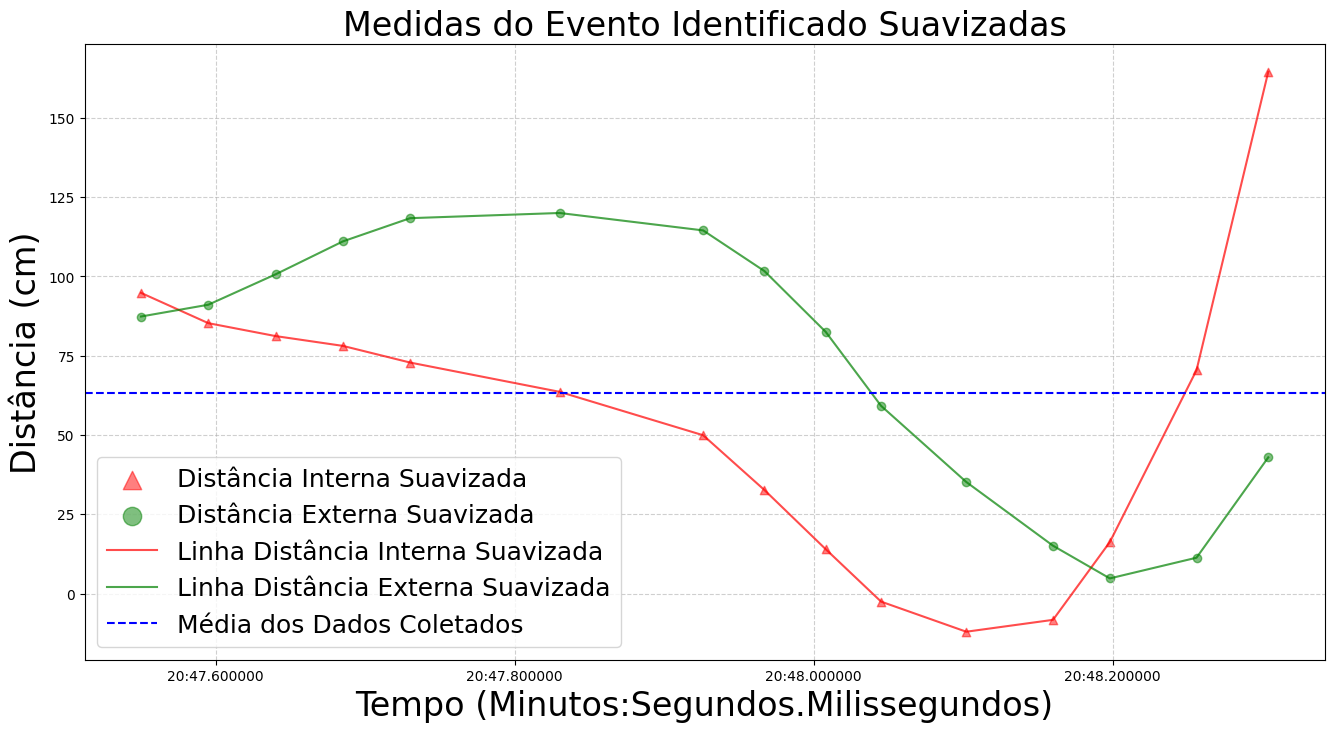
\includegraphics[width=\textwidth]{images/smoothing_ex.png}}
        \caption{Suavização das medidas de um evento}
        \label{fig:smoothing_ex}
    \end{subfigure}

    \vspace{0.4cm}

    % --- Segunda linha ---
    \begin{subfigure}[b]{0.9\textwidth}
        \centering
	    \fbox{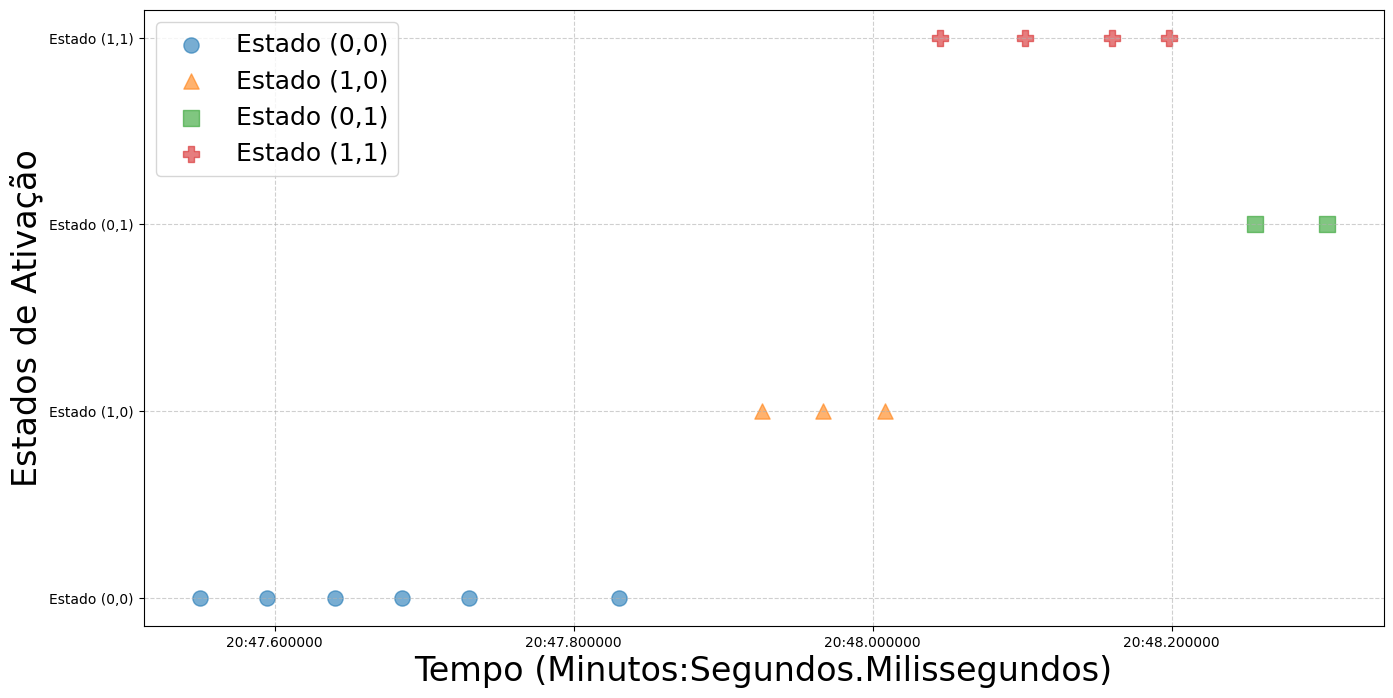
\includegraphics[width=\textwidth]{images/binarization_ex.png}}
        \caption{Estados de ativação para cada medida do evento}
        \label{fig:bin_ex}
    \end{subfigure}

    \caption{Processo de obtenção dos estados de ativação dos sensores desde a coleta de dados.}
    \label{fig:entire_cicle_ex}
\end{figure}

Após o processo de binarização disposto na Figura \ref{fig:entire_cicle_ex}, espera-se obter um conjunto de dados que permita identificar através de valores binários (0 e 1), qual a ordem de acionamento dos sensores durante possíveis eventos de interesse. Para este processo de identificação, é necessário realizar a junção dos valores binários correspondentes ao sensor externo e interno para cada medida, obtendo-se uma tupla denominada como estado de ativação do módulo de sensoriamento, assim como disposto na Figura \ref{fig:bin_ex}. Desta forma, ao identificar todos os estados de ativação que compõem o evento, bem como a ordem em que eles ocorrem, torna-se possível caracterizar o evento em uma entrada ou saída. Esse processo está descrito como Caracterização do Evento de Interesse na Figura \ref{fig:strategy_workflow} e faz uso da Tabela \ref{tab:state_machine} como modelo para análise dos eventos.

\begin{table}[H]
	\centering
	\caption{Transição de Estados do Módulo de Contagem de Pessoas}\label{tab:state_machine}
	\begin{tabular}{|c|c|c|l|}
		\hline
		\multicolumn{1}{|l|}{\textbf{Estado Inicial}} & \multicolumn{1}{l|}{\textbf{Estado Final}} & \textbf{Transições de Estados}                & \multicolumn{1}{c|}{\textbf{Descrição do evento}} \\ \hline
		(1,0)                                         & (0,1)                                      & (1,0) -\textgreater (1,1) -\textgreater (0,1) & Alguém entrou                                     \\ \hline
		(0,1)                                         & (1,0)                                      & (0,1) -\textgreater (1,1) -\textgreater (1,0) & Alguém saiu                                       \\ \hline
	\end{tabular}
\end{table}

Por fim, a etapa de caracterização consiste em analisar a sequência de estados de ativação gerada e buscar por conjuntos com ordem de acontecimentos bem definida, assim como apresentado na coluna de Transições de Estado através da Figura \ref{tab:state_machine}. Como espera-se que o algoritmo seja capaz de filtrar momentos de inatividade, o modelo utilizado para caracterizar eventos registrados não contém o estado (0,0), que corresponde a inatividade dos dois sensores ultrassônicos. Além disso, graças ao processo de suavização das medidas coletadas, caso de fato ocorra uma entrada ou saída, os valores tendem a transicionar de um estado de ativação para o outro de forma mais suave, logo o estado de ativação (1,1), que corresponde a ativação de ambos os sensores, sempre deve ocorrer, se tornando um estado ativação em comum entre os dois eventos e essencial para eventos válidos.



%%Fim da seção de abordagem proposta

%%Início da seção de implementação da abordagem evoluída
\subsection{Implementação do Módulo Evoluído}
\label{subsec:module_implementation}
Após elaborar a sequência de etapas que demonstrou performance promissora no pré-tramento dos dados coletados pelo dispositivo BIoT, e consequentemente um melhor reconhecimento de eventos de interesse, é necessário realizar a implementação da abordagem evoluída no contexto do sistema SAFE/UFRJ, para que seu funcionamento seja avaliado em conformidade com todo os subsistemas que compõem a aplicação IoT. Deste modo, a presente subseção pretende descrever todo o processo de evolução dos componentes de \textit{software}, bem como as decisões arquiteturais adotadas tendo em vista o ambiente de desenvolvimento embarcado, no qual sistemas de \textit{software} IoT se enquadram.

Atualmente, o dispositivo BIoT é composto por um microcontrolador ESP32 conectado há uma coletânea de sensores encarregados de coletar informações sobre a qualidade do ar interno e monitorar o fluxo de pessoas em uma instalação \cite{SAFE-IOT}. Para o desenvolvimento em embarcados, o uso de memória e processamento requer mais atenção, tendo em vista que este tipo de \textit{hardware} possui recursos mais limitados que estações de trabalho convencionais. O ESP32 pode ser considerado um microcontrolador poderoso, pois dispõe de um processador com dois núcleos, 520 Kbytes(KB) de memória SRAM(\textit{Static Random Acess Memory)}, 448KB de memória ROM(\textit{Read-only Memory} e 4 Megabytes(MB) destinados a memória Flash \cite{hercog_design_2023}. Além disso, esta placa de desenvolvimento apresenta módulos de Wi-Fi e Bluetooth de fábrica, facilitando a implementação de comunicação sem fio, um requisito para implementações IoT \cite{motta_evidence-based_2023}.

A arquitetura \textit{dual-core} do microcontrolador em uso, possibilitou que o \textit{software} desenvolvido para o BIoT, fosse implementado através de paradigmas de computação concorrente, como estratégias \textit{lock-free}, para a alocação dinâmica de memória e políticas de escalonamento de tarefas \cite{kim_lwmalloc_2025, lee_fast_2011}. Estas decisões arquiteturais foram mantidas durante a evolução do dispositivo. Deste modo, todas as funções implementadas, que configuram a evolução do BIoT, seguem as mesmas regras de modelagem e desenvolvimento, um exemplo é a Figura \ref{fig:get_ultrassonic_measures_workflow}, a qual apresenta a sequência de etapas que constituem a tarefa de coleta e armazenamento de medidas, todo este processo é executado por um núcleo arbitrário designado pelo escalonador de tarefas.

\begin{figure}[H]
    \centering
    \fbox{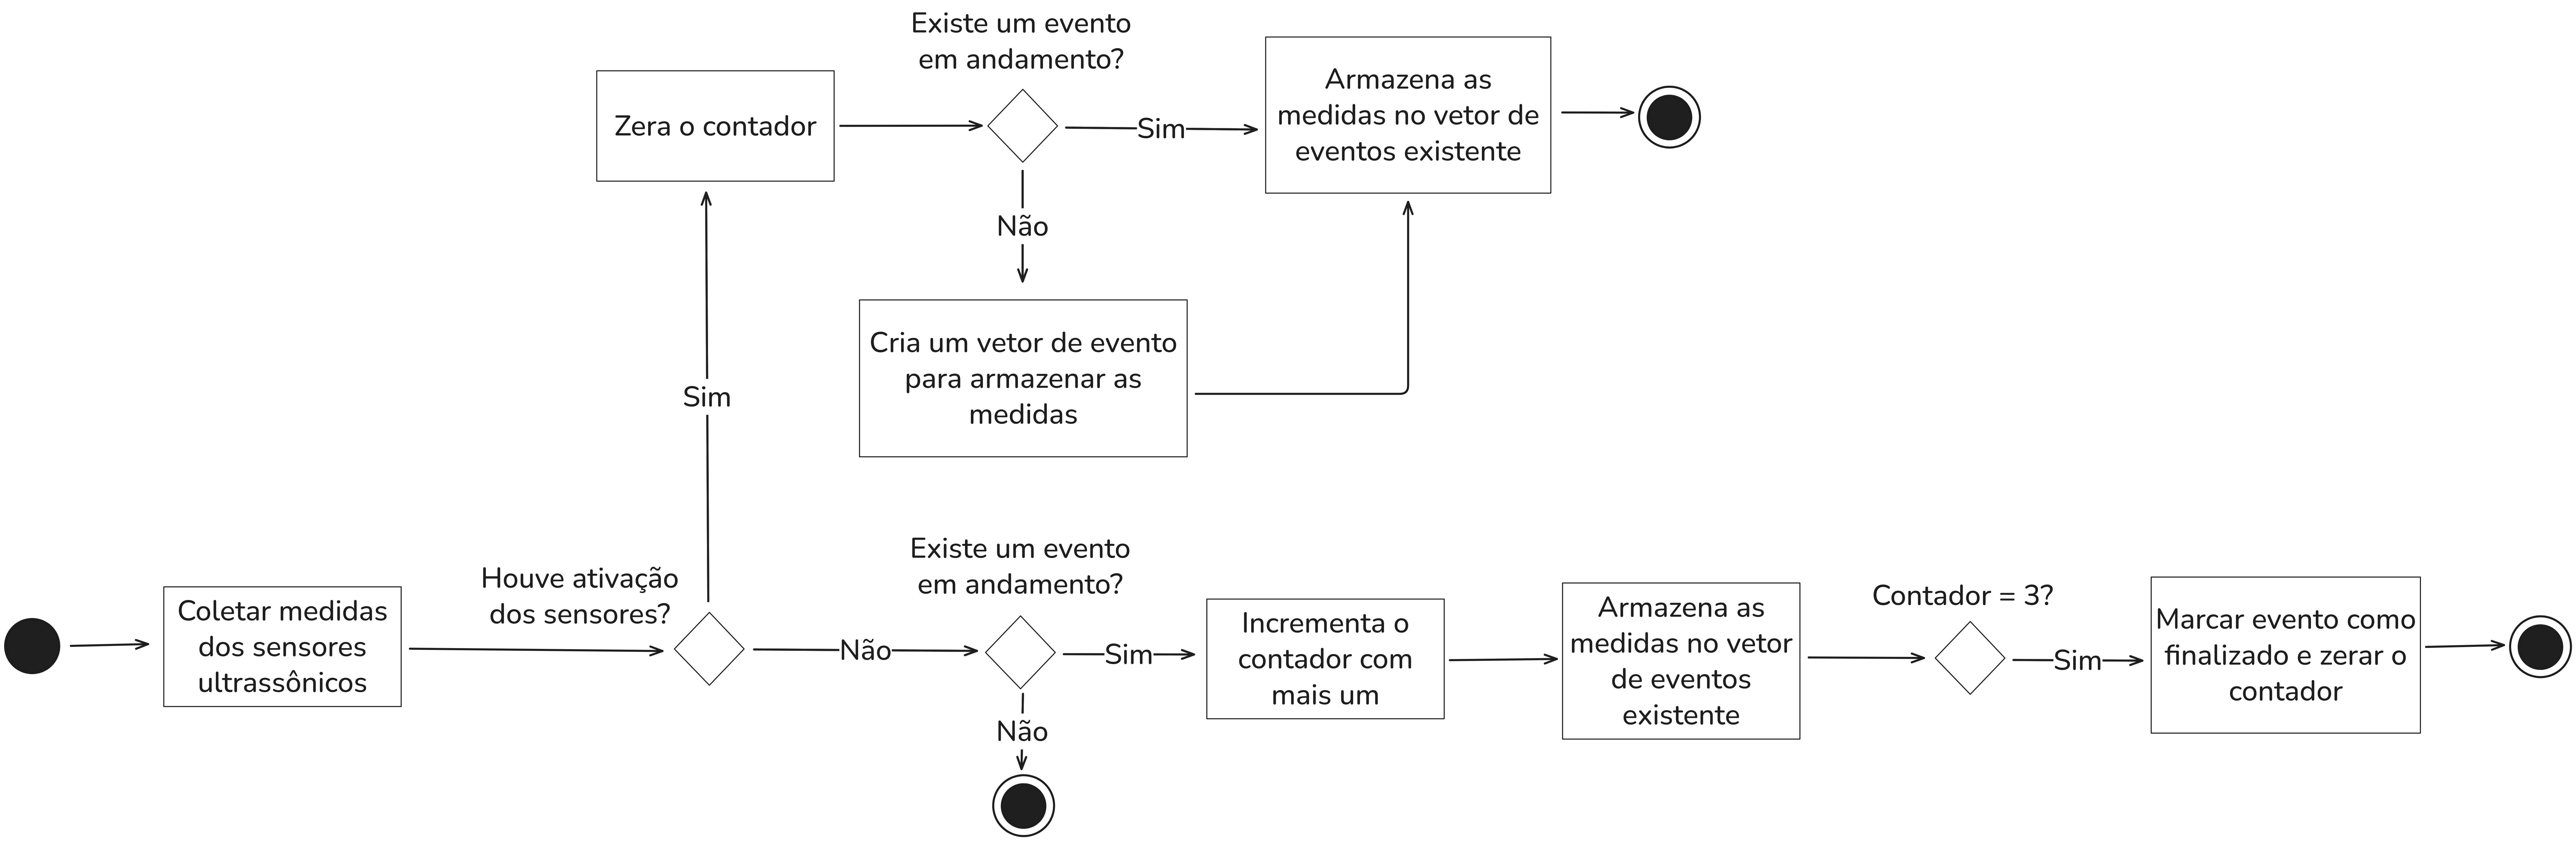
\includegraphics[width=\linewidth]{images/fluxograma_coleta_medidas_hcsr04.png}}
    \caption{Fluxo de construção de eventos de interesse}
    \label{fig:get_ultrassonic_measures_workflow}
\end{figure}

O processo de construir estruturas de dados, para armazenar medidas que compõem um possível evento de interesse, consiste nas primeiras duas etapas da estratégia de contagem de pessoas descrita previamente na Subseção \ref{subsec:module_evolution}. Entretanto, diferentemente do contexto de elaboração da abordagem, onde o \textit{dataset} submetido ao pré-tratamento é antecipadamente coletado, na circunstância da aplicação este conjunto de dados é construído de forma incremental e síncrona medida por dedida. O fluxograma presente na Figura \ref{fig:get_ultrassonic_measures_workflow} apresenta toda lógica de inclusão das medidas para composição de um evento. Em síntese, para cada ativação de um dos sensores, o dispositivo acumula medidas em um vetor até que sejam detectados três períodos consecutivos de inatividade, de acordo com as condições destacadas na subseção anterior, após isso o vetor recebe uma etiqueta que sinaliza para a tarefa em espera, que aquele grupo de dados está pronto para a próxima etapa, bem como pode conter um evento de interesse. 

\begin{figure}[H]
    \centering
    \fbox{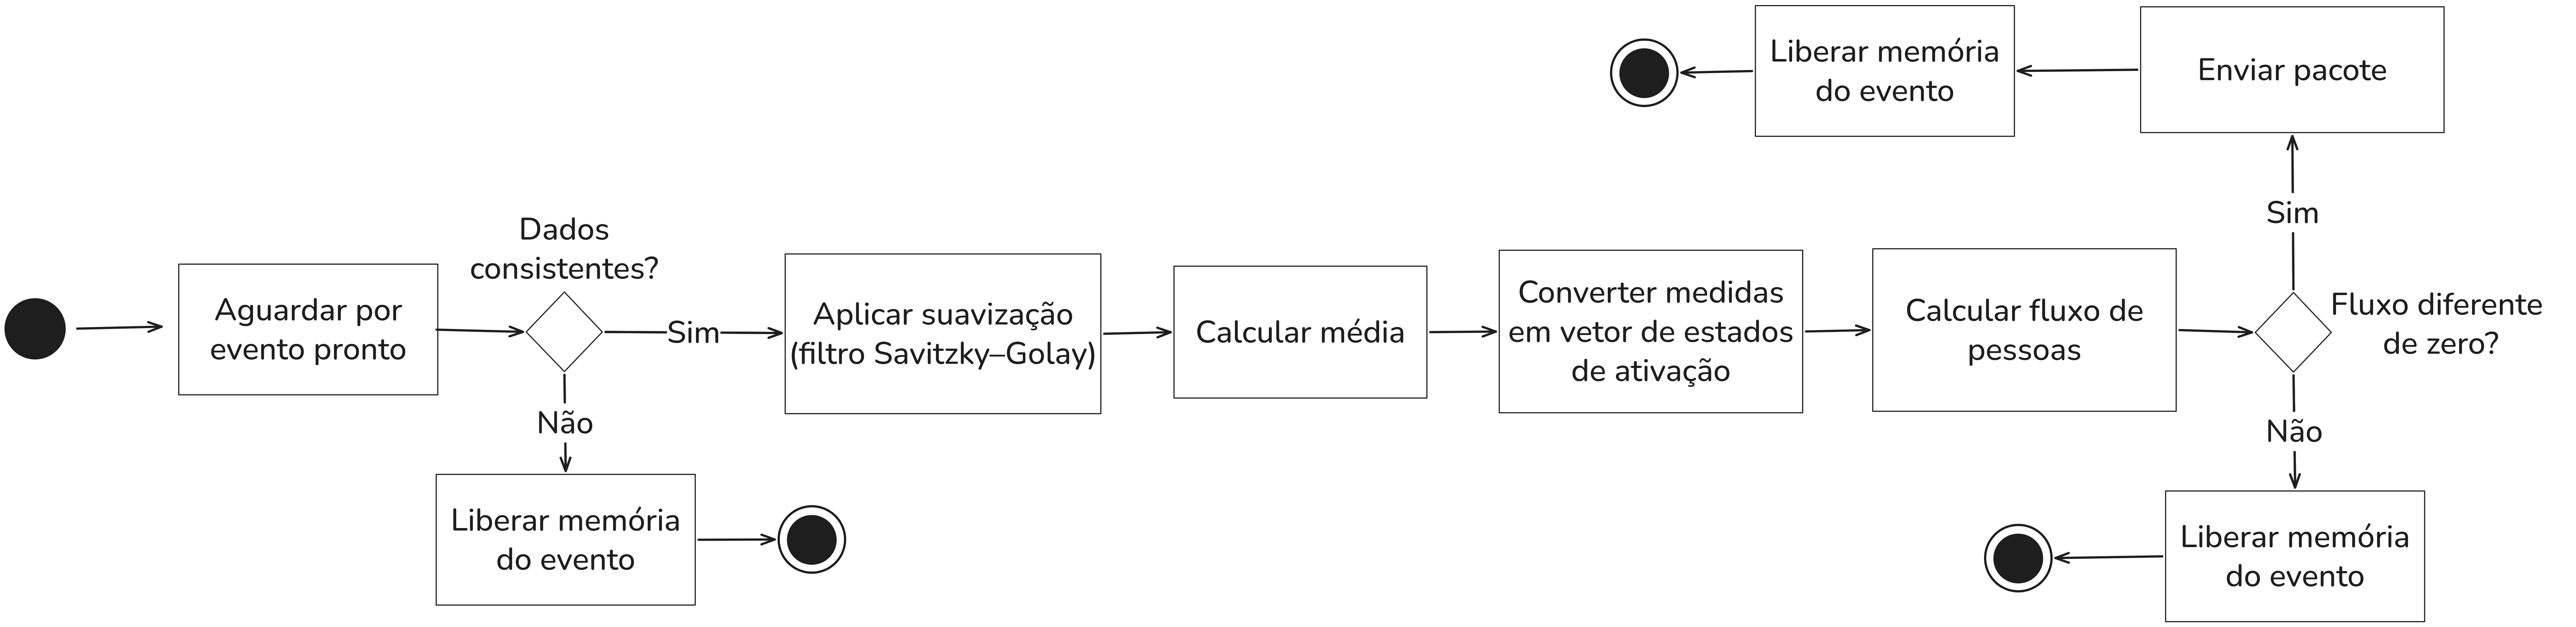
\includegraphics[width=\linewidth]{images/fluxograma_tarefa_consumo_eventos.png}}
    \caption{Sequência de atividades para calcular o fluxo de pessoas em eventos registrados}
    \label{fig:get_events_workflow}
\end{figure}

Após a atribuição do status de pronto ao evento, o vetor de medidas permanece em espera até que o escalonador execute o procedimento responsável pelo cálculo do fluxo de pessoas. A Figura \ref{fig:get_events_workflow} apresenta o fluxograma dessa tarefa, cujo objetivo é complementar as etapas da estratégia previamente descrita na Subseção \ref{subsec:module_evolution}. Assim, as atividades representadas correspondem majoritariamente a processos já detalhados, com exceção da liberação de memória associada à alocação dinâmica e do envio de pacotes, referentes à comunicação sem fio do dispositivo BIoT para publicação das medidas. Destaca-se ainda a etapa de suavização dos dados, implementada por meio de uma biblioteca adaptada exclusivamente para os requisitos do sistema. O Algoritmo \ref{alg:suavizacao_sg_nearest} descreve de forma mais rigorosa a lógica de funcionamento desse componente.

\begin{algorithm}[H]
\caption{Suavização Savitzky--Golay com bordas por vizinho mais próximo}
\label{alg:suavizacao_sg_nearest}
\begin{algorithmic}[1]
\Require vetor de entrada $x[0..L-1]$, vetor de saída $y[0..L-1]$, $L$, $janela$, $ordemPol$
\Ensure $y$ preenchido com a série suavizada, ou falha
\Function{SuavizarSG}{$x,y,L,janela,ordemPol$}

  \If{$x=\textsc{null}$ \textbf{or} $y=\textsc{null}$ \textbf{or} $L=0$}
    \State \Return \textbf{false} \Comment{Validação de ponteiros e tamanho}
  \EndIf

  \State $janela \gets \Call{AjustarJanela}{L,janela}$ \Comment{Força $3 \le janela \le 21$ e ímpar}
  \If{$janela < 3$ \textbf{or} $janela > 21$ \textbf{or} $janela$ é par}
    \State \Return \textbf{false} \Comment{Janela inválida após ajuste}
  \EndIf

  \State $ordemPol \gets \min(5,\max(2,ordemPol))$ \Comment{Limita a ordem polinomial em $[2,5]$}
  \If{$janela < 4$}
    \State $ordemPol \gets 2$ \Comment{Regra: janela muito curta força ordem 2}
  \EndIf

  \State $linha \gets (janela-3)/2$ \Comment{Mapeia janela (3..21) para linha na tabela}
  \State $coef \gets \begin{cases}
	  CoefSG_{P3}[\textit{linha}], & \text{se } ordemPol \le 3\\
	  CoefSG_{P5}[\textit{linha}], & \text{caso contrário}
  \end{cases}$ \Comment{Escolha da tabela de coeficientes}

  \State $M \gets \lfloor janela/2 \rfloor$ \Comment{Semi-janela: amostras em cada lado}
  \State $ultimo \gets L-1$ \Comment{Último índice válido}
  \State $denom \gets coef[0]$ \Comment{Denominador (normalização)}

  \For{$n \gets 0$ \textbf{to} $L-1$}
    \State $acum \gets coef[1+M]\cdot x[n]$ \Comment{Peso do centro ($k=0$)}
    \For{$k \gets 1$ \textbf{to} $M$}
      \State $h \gets coef[1+(M-k)]$ \Comment{Peso simétrico para distância $k$}
      \State $i_m \gets \Call{Limitar}{n-k,0,ultimo}$ \Comment{Borda: satura índice à esquerda}
      \State $i_p \gets \Call{Limitar}{n+k,0,ultimo}$ \Comment{Borda: satura índice à direita}
      \State $acum \gets acum + h\cdot (x[i_m] + x[i_p])$ \Comment{Soma par simétrico}
    \EndFor
    \State $y[n] \gets acum/denom$ \Comment{Normaliza e grava a saída}
  \EndFor

  \State \Return \textbf{true} \Comment{Suavização concluída}
\EndFunction
\end{algorithmic}
\end{algorithm}

A implementação do filtro de Savitsky-Golay foi realizada em conformidade com as equações X e Y previamente discutidas na subseção anterior. No entanto, o componente possui algumas particularidades devido ao contexto da aplicação, como restrições da ordem do polimônio e limites bem definidos para o tamanho da janela de suavização. A imposição deste tipo de restrição tem como objetivo, prevenir que o algoritmo adote configurações que podem impedir ou prejudicar a suavização dos dados e consequentemente o cálculo do fluxo de pessoas. Por fim, destaca-se que todas delimitações foram obtidas de forma experimental através dos estudos realizados durante a etapa de análise exploratória dos dados e avaliação da estratégia evoluída. 


Para realizar estas restrições duas funções foram implementadas, ``AjustarJanela'' e ``Limitar'', a primeira função tem como objetivo garantir que o tamanho da janela de suavização sempre esteja dentro do limite fechado $[3..21]$ e corresponda a um valor ímpar, esta última limitação é herdada da formulação matemática do filtro de SG e é necessária para que ele atue como o esperado. A segunda função, representa o método adotado para lidar com os valores que estão na borda do conjunto de medidas, como o filtro adotado realiza somas simétricas em torno da posição central ($n+k$ e $n-k$), nas regiões próximas ao início ou fim do vetor, estes índices podem se tornar negativos ou superiores ao tamanho do conjunto de medidas ($L-1$). A operação de saturação, impede que isso aconteça substituindo os valores fora do intervalo pelo índice válido mais próximo, esta estratégia é conhecida como tratamento de bordas por vizinho mais próximo (\textit{nearest boundary condition}). Este método foi adotado pois confere aos valores brutos inicias e finais maior impacto no cálculo de influência, isto é positivo para o desempenho da aplicação, pois normalmente estas medidas correspondem a variações de estado, logo devem ser percebidas de forma clara pelo algoritmo. 

Por fim, destaca-se, as principais implicações da evolução do dispositivo BIoT e as consequentes mudanças estruturais do sistema. Em sua versão inicial, o dispositivo BIoT realizava a publicação de medidas de forma bruta, sem nenhum pré-tratamento, transferindo toda a responsabilidade de acúmulo de medidas e cálculo de fluxo de pessoas, para o subsistema encarregado de consumir as mensagens publicadas. O novo módulo de contagem de pessoas, realiza a coleta, processamento e análise das medidas de forma completamente embarcada, isto é, a nível de dispositivo, enviando como medida apenas a variação de indivíduos em uma instalação. Deste modo, o dispositivo passa a enviar mensagens mais inteligentes[IoT Roadmap] e menores, além de extinguir a necessidade de envio e acúmulo de medidas brutas.


%%Fim da seção de implementação da abordagem evoluída
